%!TEX root = Main.tex
\documentclass[Main]{subfiles}

\begin{document}

\section{Design, implementation and test setup} % (fold)
\label{sec:design_implementation_test_setup}

	\subsection{System Description}
		The main functional blocks of the system are shown in Figure \ref{fig:sysDesc}. 
		CO$_2$ emission data is acquired from the FTP server by the Java application. The Java application determines whether the emission is high or low and transmits the corresponding control message to the ZigBee LED device. 
		The Sequence Executor Tool is used by the Java application for managing the communication with the ZigBee LED device. 
		By specifying the address of the SmartAMM server, ZigBee gateway ID and ZigBee LED device ID, the Java application is able to communicate with the ZigBee LED device.  

		\begin{figure}[H]
		\centering
		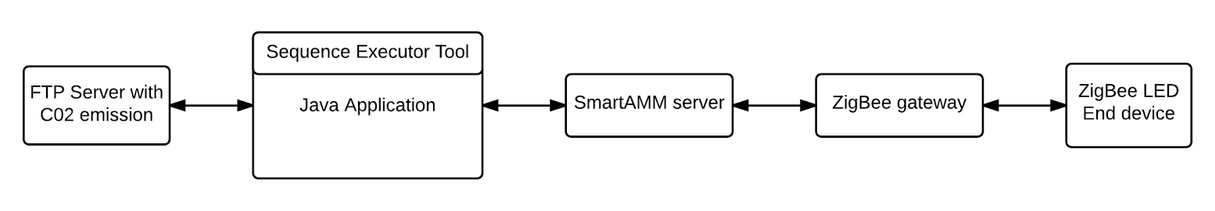
\includegraphics[width=\linewidth]{SystemDescription}
		\caption{System description}
		\label{fig:sysDesc}
		\end{figure}




	\subsection{Decision Making}



	\subsection{Sequence Executor Tool}
		The Sequence Executor Tool, which is provided by Develco Products, is a Java application able to communicate with ZigBee devices through a SmartAMM server.
		It requires two input files: A \emph{setting} file and a \emph{sequence} file.

		The \emph{settings} file is a XML file that contains various settings used in the tool. 
		The most relevant is settings regarding which server the tool should connect to. 
		In this project, the server was hosted on a local PC and the gateway was a USB dongle, which resulted in the following settings:
		\begin{itemize}
			\item gatewayType: ActiveMQ
			\item portNo: 62000
			\item hostName: localhost
		\end{itemize}

		The \emph{sequence} file is also an XML file, specifying the sequence of telegrams to be sent to the ZigBee device, including gateway and device IDs. 
		It also specifies how to determine whether the telegram was successfully receive. 
		In this project positive acknowledgment are used as an indicator for successful transmission.
		In \ref{sec:appendix_a} the XML files for authorizing the ZigBee end device on the network, and setting the LED green is shown.
		Each sequence file contains the following items: 
		\begin{itemize}
			\item General sequence descriptions
			\item Substitute texts
			\item Steps
		\end{itemize}
		The general description contains information like sequence name, author, tool version etc.
		The substitute texts are a smart feature in the tool. 
		These allows the user to easily change certain fields in the steps. 
		A great example of this is the sequence file specifying setting the LED red or green.
		Instead 




	\subsection{Application}



	\subsection{Communication Protocols}
		% Zigbee - Ivan Starter
		% Web protokoller - Ivan Starter
		% Det sidste



% section design_implementation_test_setup (end)
\end{document}